%%%%%%%%%%%%%%%%%%%%%%%%%%%%%%%%%%%%%%%%%%%%%%%%
% 1: Introducción
%%%%%%%%%%%%%%%%%%%%%%%%%%%%%%%%%%%%%%%%%%%%%%%%
\pagenumbering{arabic} % para empezar la numeración con números
\chapter{Introducción}
\label{introduccion}


%Desde el comienzo de su historia, la informática ha intervenido en cada aspecto científico y social existente. La dependencia de la sociedad en una ciencia tan reciente resalta la importancia de que sea algo comprensible y comprendido para la sociedad misma.

Como dice M. Lemaire\cite{lemaire2014incorporating}, en una sociedad que está incrementando su dependencia a las nuevas tecnologías\footnote{Aquí, con nuevas tecnologías me refiero a productos y proyectos derivados de la Informática y las \acrfull{TIC} como puede ser los proyectos que detallamos en la sección \ref{estado-arte}.}, es imprescindible que las nuevas generaciones desarrollen la habilidad de pensar de manera crítica sobre tecnología.

El \emph{Computational Thinking} (pensamiento computacional)\cite{wing2006computational}, es el arte de pensar como un ordenador. El pensamiento computacional, como se refiere A. Bundy en \cite{bundy2007computational}, afecta a investigaciones de casi todas las disciplinas, tanto de ciencias como de humanidades. [...] La informática no solo ha permitido que los investigadores puedan hacer nuevas preguntas, sino también ha permitido aceptar nuevos tipos de respuesta. Por ejemplo, preguntas que requieren el procesamiento de una gran cantidad de datos.

Es necesario comprender la informática y desarrollar el \emph{pensamiento computacional}. Se necesitan desarrollar nuevas tecnologías, nuevo \gls{hardware} y \gls{software} que automatice tareas largas, complejas y con una alta cantidad de cómputo. Tareas que no siempre los humanos podemos resolver de manera directa. Para conseguir esto, muchas veces es necesario programar.


Pero aprender a programar es mencionado como uno de los 7 grandes retos de la educación informática \cite{mcgettrick2005grand} y diversos estudios \cite{renumol2009classification} muestran que las principales dificultades para un alumno cuando está en el proceso de aprender a programar son (a) como empezar un programa; (b) comprensión de la sintaxis específica del lenguaje de programación; (c) comprensión de la lógica\footnote{En este caso me refiero a lógica booleana, o también llamada Álgebra de Boole.} y (d) problemas a la hora de depurar el código escrito.

Aunque a primera vista aprender a programar pueda parecer una tarea ardua y compleja, tiene sus ventajas. En el estudio realizado por J. Siegmund y otros en \cite{siegmund2014understanding}, se puede ver como los participantes mientras comprendían, analizaban y buscaban errores en pequeños trozos de código, daban claras muestras de estar desarrollando actividad cerebral en regiones del cerebro relacionadas con el procesado del lenguaje, la atención y la memoria de trabajo.

De la misma manera, estudios realizados en niños \cite{clements1986effects} de entre 6 y 8 años, muestran que estos demostraron mayor capacidad de atención, más autonomía y un mayor placer por el descubrimiento de nuevos conceptos. En la misma linea, un estudio en niños de infantil \cite{logo-geometry} que utilizaban el \Gls{logo} demostró que los mismos obtuvieron mejores resultados en pruebas de razonamiento, matemáticas o resolución de problemas. Otro estudio más reciernte \cite{liao1991effects} demuestra que aprender a programar (independientemente del lenguaje) a una corta edad, potencia la creatividad y la habilidad de aprendizaje.



\section{Situación actual}
\label{sec:situacion-actual}


Actualmente existen muchos proyectos con el fin de introducir la programación como asignatura obligatoria en Educación Primaria y Secundaria\footnote{En este documento se hablará a menudo de alumnos de Educación Primaria, Secundaria o Bachillerato pero no siempre referido al sistema educativo español. Cada pais tiene un sistema educativo diferente que varía la edad de escolarización de los alumnos. Por generalizar, se tomará la edad y cursos escolares como referencia cuando se hable de Educación Primaria, Secundaria o Bachillerato. En el Apéndice \ref{anexo:edad-educacion} se profundiza más en la diferencia de edad en los principales Sistemas Educativos que pueden ser referenciados, directa o indirectamente, en el presente documento.}. Estos proyectos vienen respaldados por importantes cambios en los planes de estudios de todo el mundo para enseñar programación\cite{cs-education,madrid-programacion,codigo21, guide-england-computing,chicago-cs}, marcando una clara tendencia social de incluir la programación en los currículos académicos.


Uno de los proyectos más importantes y con más repercusión a nivel global es Code.org\cite{code-org}. Propone una serie de herramientas y juegos diseñados especialmente para que los niños aprendan programación mientras juegan con sus personajes favoritos de películas y videojuegos. Todo ello acompañado de una infraestructura para que profesores puedan incluir estos proyectos en las aulas, y padres en sus casas.
Su proyecto \emph{Hora del código}\cite{hour-of-code} consigue reunir a niños de todas las edades una hora al día para que la inviertan en programar.
Code.org cuenta con decenas de millones de estudiantes de más de 180 países, disponible en más de 30 idiomas. De manera gratuita, cualquiera puede aprender a programar en eventos que se realizan por todo el mundo (figura \ref{fig:map-hour-code}). Code.org está apoyado por grandes compañías y persanalidades a nivel global como puede ser Microsoft, Google, el Presidente Barack Obama, Mark Zuckerberg, Bill Gates o Walt Disney Company. {\color{gree}En la sección \ref{sec:Code.org} se abordará más detalladamente las diferentes formas que tiene Code.org de enseñar a programar.}


\begin{figure}[!ht]
	\begin{centering}
		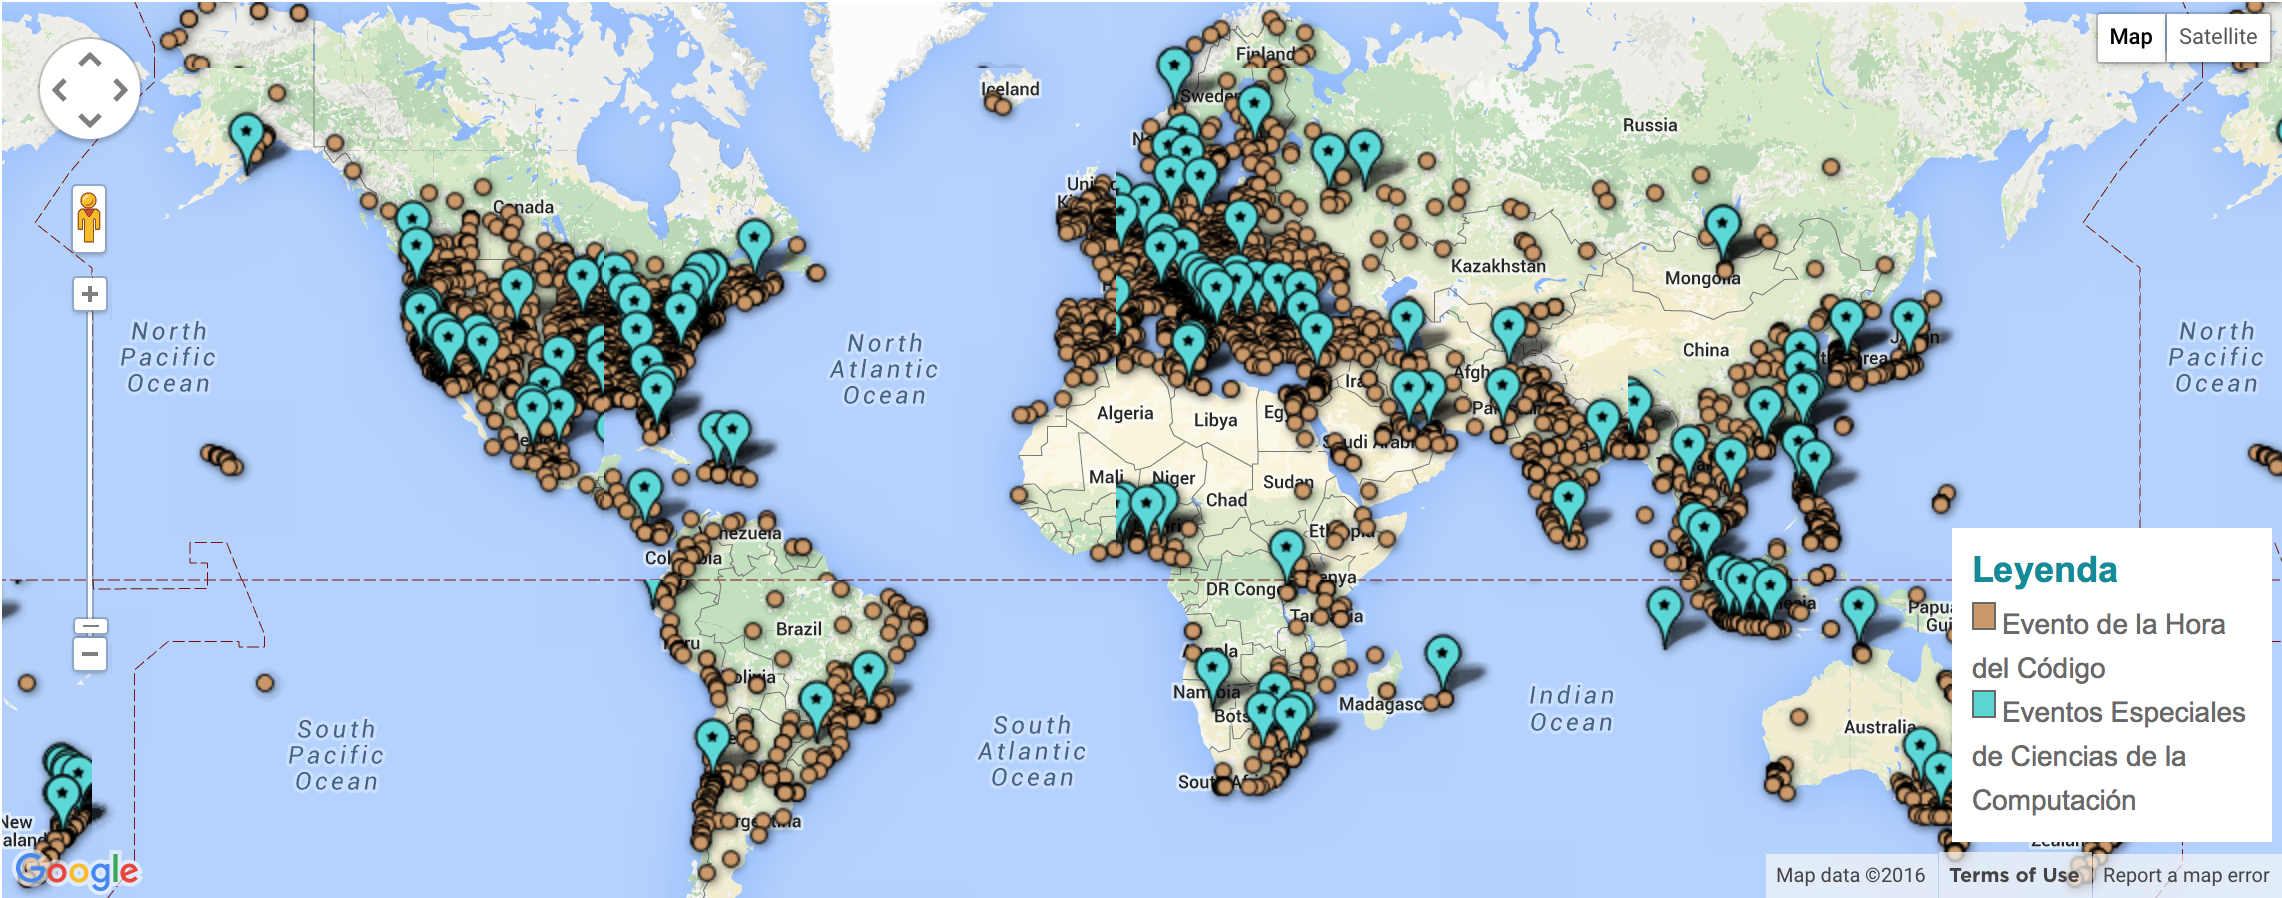
\includegraphics[width=0.8\textwidth]{images/map-hour-code.png}
			\caption{Mapa de visualización de eventos de llevados a cabo por el proyecto \emph{Hora del código} alrededor del mundo. Actualmente 198,473 en todo el mundo, 1,839 en España. Obtenido de \cite{hour-of-code}.}
				\label{fig:map-hour-code}
	\end{centering}
\end{figure}


A nivel europeo, la \Gls{com-euro}\cite{ec-code-week} ha promovido durante el año 2015 la \emph{EU Code Week}\cite{code-week} como parte de su Estrategia para la Educación y la Formación 2020. Este proyecto consistió en eventos de una semana de duración en la que se enseñaba informática y programación en lugares de toda Europa\footnote{En España, se realizaron eventos dentro del marco del proyecto \emph{EU Code Week} en Madrid, Sevilla, Murcia, Asturias, Canarias, Cantabria, Zamora, Cataluña, Ceuta, Badajoz, La Rioja, País Vasco y Valencia.}.


\section{La robótica como herramienta de aprendizaje}
\label{sec:electronica-robotica}


Es bastante común que la introducción en las aulas del \emph{Computational Thinking} sea a través de la robótica y electrónica. Muchos proyectos de robótica animan al alumno a formarse en dos grandes materias: electrónica y programación. Cuando un estudiante tiene que hacer que un robot se mueva, tendrá que aprender a programar su comportamiento, pero también deberá conocer y en algunos casos incluso crear nuevas piezas para su correcto funcionamiento y personalización.

Existen proyectos como Arduino\cite{arduino} y Raspberry Pi\cite{raspberry-pi} que proporcionan los elementos y materiales básicos para poder crear nuevos proyectos. Arduino es una placa base con un microprocesador que es capaz de analizar entradas de información (un sensor, un botón o incluso una notificación de Twitter (\url{www.twitter.com}) y convertirlo en una respuesta como el activar un robot o encender un led. Todo esto acompañado de un software facil de programar. El proyecto es completamente \emph{\gls{open-source}}. Raspberry Pi es un ordenador del tamaño de una tarjeta de crédito. También se provee por defecto un Sistema Operativo \emph{Open Source} pero el sistema está completamente abierto a cambios y mejoras por parte de la comunidad. 


En concreto, una de las meta originales de Raspberry Pi es conseguir que los niños aprendan a programar y conozcan como funciona realmente un ordenador. Tanto Arduino como Raspberry Pi pueden adquirirse a un bajo precio, lo que facilita que las instituciones de enseñanza introduzcan estas tecnologías en las aulas como parte de su currículo.


Otro proyecto que también está muy extendido en las aulas es Lego Mindstorm EV3 y NXT\cite{lego-mindstorm}. Dos kits de iniciación a la robótica con Lego. Permite al estudiante crear con piezas de lego un robot y programar su comportamiento. Los robots suelen tomar forma de brazo robótico o de vehículo capaz de seguir lineas pintadas en el suelo haciendo uso de sensores. Toda este material robótico viene acompañado de un software para programar el comportamiento de los diferentes componentes del robot y un estilo de programación con bloques\cite{lego-mindstorm-programar}, similar al usado en Scratch.

En la sección \ref{sec:aprendiendo-robots} se hablará más del uso de la electrónica y la robótica como elementos de enseñanza.



\section{Proyecto Descubre la programación}
\label{sec:descubre}

\Gls{descubre}\cite{descubre} es un proyecto diseñado en la Facultad de Informática de la Universidad de Murcia y tiene como objetivo ayudar a los alumnos de Secundaria y Bachillerato a que desarrollen sus capacidades descubriendo lo que es la informática y aprendiendo a programar. Así como fomentar la inclusión del aprendizaje de la programación en secundaria y bachillerato.

Para ello, en un mismo sitio web, se integra (a) un conjunto de tutoriales de programación; (b) una herramienta que permite programar (figura \ref{fig:descubre-crea}) y realizar ejercicios o retos propuestos y (c) una pequeña red social que permite publicar y compartir con el resto de compañeros los programas realizados. Adiccionalmente se puede consultar las estadísticas de aprendizaje y tiempo dedicado en la plataforma, tanto por el alumno como por el profesor. De esta manera se permite que los profesores puedan utilizar Descubre en las aulas y realizar un seguimiento de la dedicación y progreso del alumno.

En cuanto a la herramienta para desarrollar programas, el lenguaje utilizado es \gls{ijava}\cite{sanchez2009ijava} y ha sido desarrollado por J. A. Sánchez Laguna. iJava es un lenguaje imperativo basado en \Gls{java} que comparte su sintaxis. Ofrece un enfoque procedural para programar con la Orientación a Objetos como algo opcional.
% aunque se han eliminado todos los componentes del lenguaje Orientado a Objetos. 
 También incorpora un conjunto reducido de funciones de librería clasificadas en los tres grupos siguientes: númericas, entrad/salida y gráficas\footnote{Si el lector está interesado en aprender más sobre este lenguaje, puede consultar \cite{sanchez2009ijava} o \cite{descubre-lenguaje}.}.

A modo de ilustración, podemos ver el código \ref{code:hello-world}, un programa que imprime por pantalla la cadena "Hello World". En el código \ref{code:circulos-color-raton} podemos ver un programa un poco más complejo que dibuja círculos de colores en la pantalla según la posición del ratón. En la figura \ref{fig:salida-code-circulos-color-raton} se puede ver la salida de este último programa.


\begin{lstlisting}[language={Java}, label={code:hello-world}, caption={Programa básico en iJava imprimiendo la cadena "Hello World".}]
void main(){
  print("Hello World");
}
\end{lstlisting}


\begin{lstlisting}[language={Java},label={code:circulos-color-raton}, caption={Programa en iJava que dibuja un circulo de un color diferente según la posición en la pantalla en la que se encuentra el ratón.}]
void main() {
  //repetimos en bucle la funcion 'draw'
  animate(draw);
}

void draw() {
  //coloreamos el circulo segun la posición del raton
  fill(mouseX, mouseY, 0); //valores RGB
  //dibujamos una elipse con radio 50
  ellipse(mouseX, mouseY, 50,50);
}
\end{lstlisting}


La sintaxis de iJava se parece a muchos de los lenguajes modernos y más utilizados (al ser un subconjunto de la sintaxis de Java), lo cual simplifica el aprendizaje cuando se intenta aprender un nuevo lenguaje. También, gracias a la librería gráfica y matemática, los programas se simplifican mucho en cuanto a complejidad y longitud. De esta manera se consigue aligerar la carga de trabajo que tiene que realizar el alumno para conseguir hacer un programa vistoso, haciendo que la actividad de programar sea más atractiva.


\begin{figure}[!ht]
	\begin{centering}
		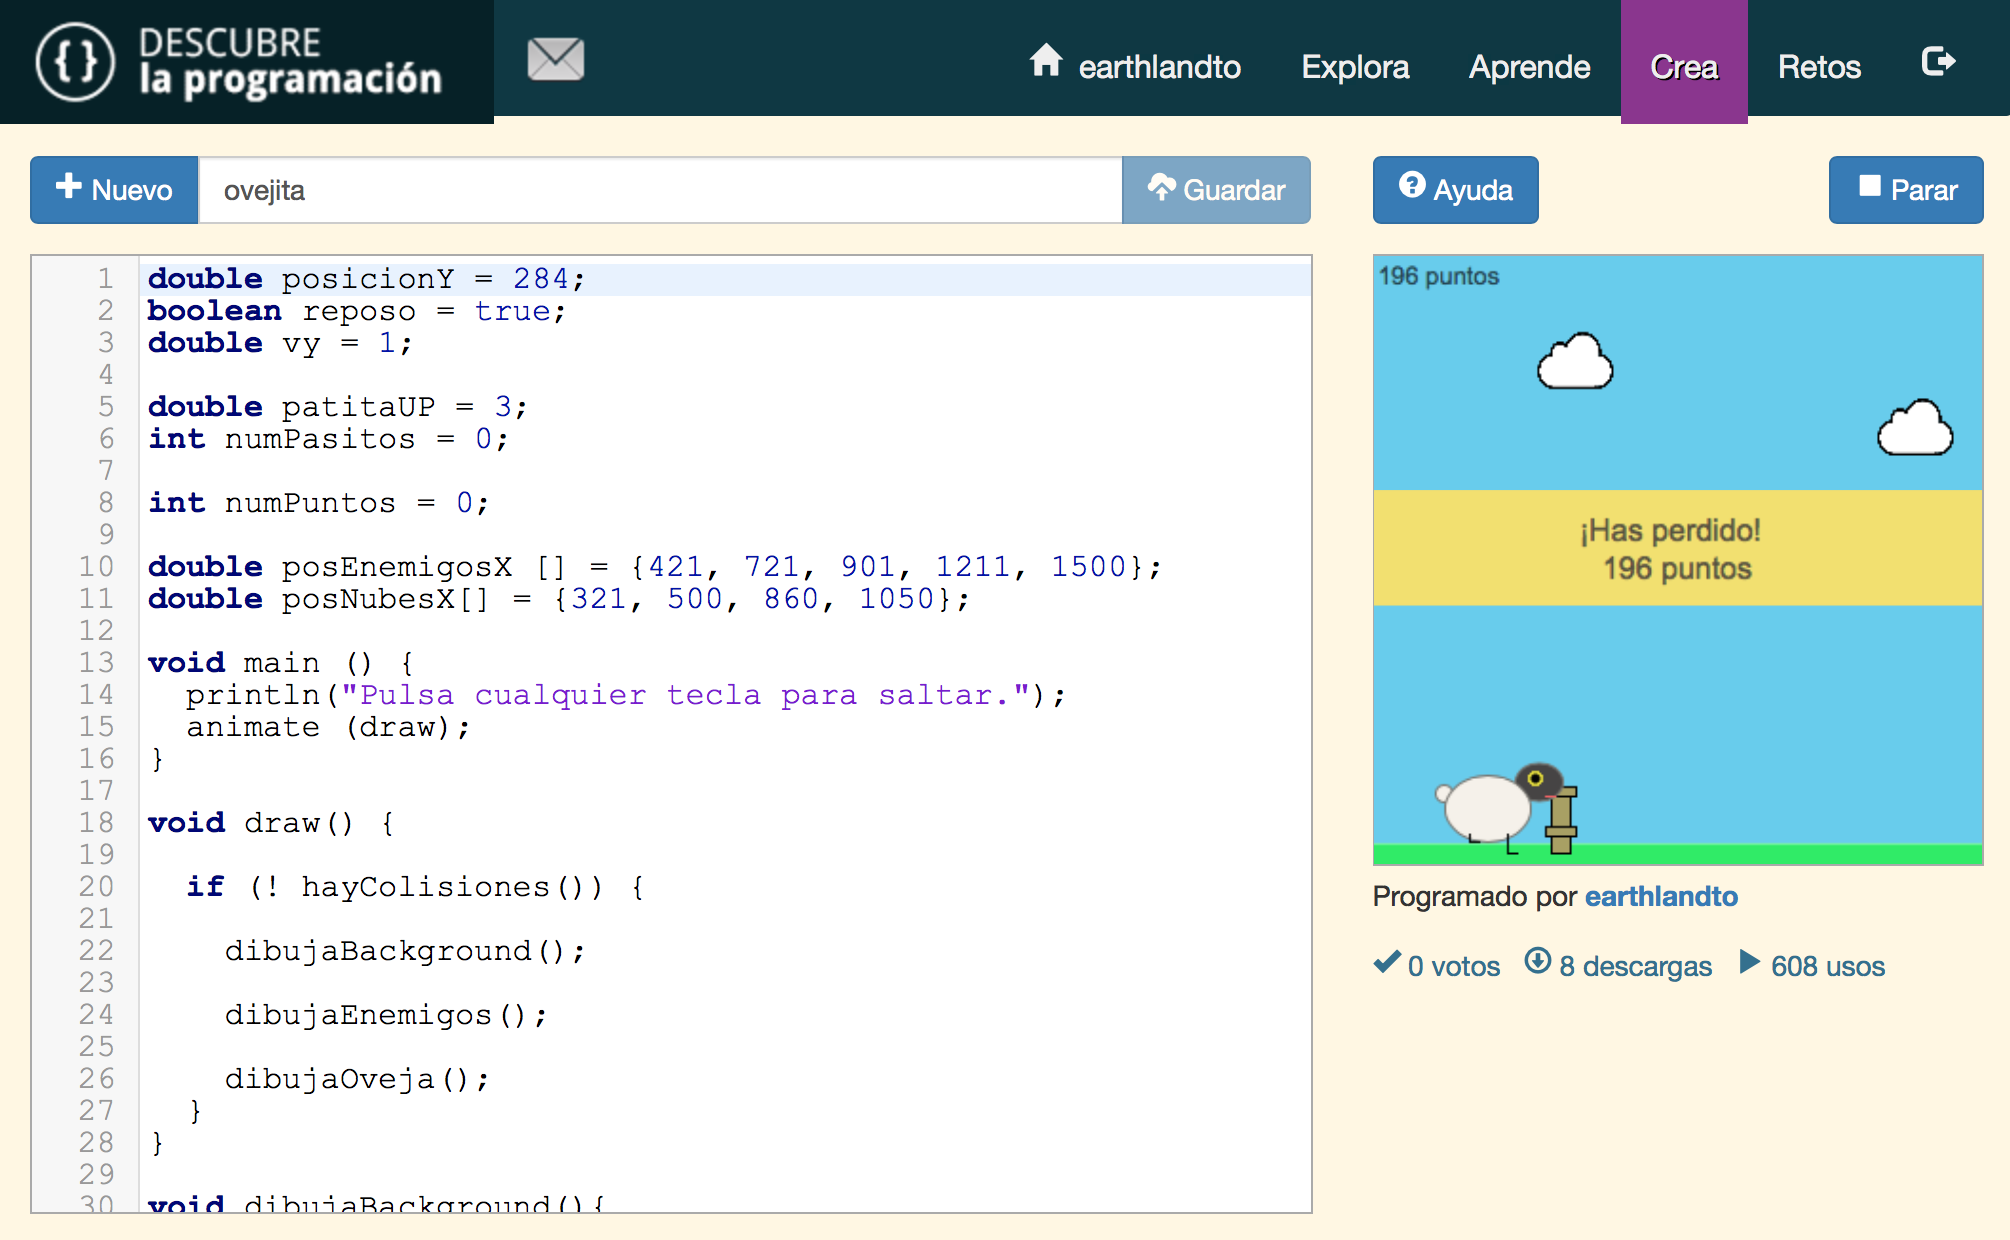
\includegraphics[width=0.7\textwidth]{images/descubre-crea.png}
				\caption{Sección \emph{Crea} del proyecto \Gls{descubre}. Obtenido de \cite{descubre}.}
				\label{fig:descubre-crea}
	\end{centering}
\end{figure}


% 
% \begin{figure}[!ht]
% 	\begin{centering}
% 		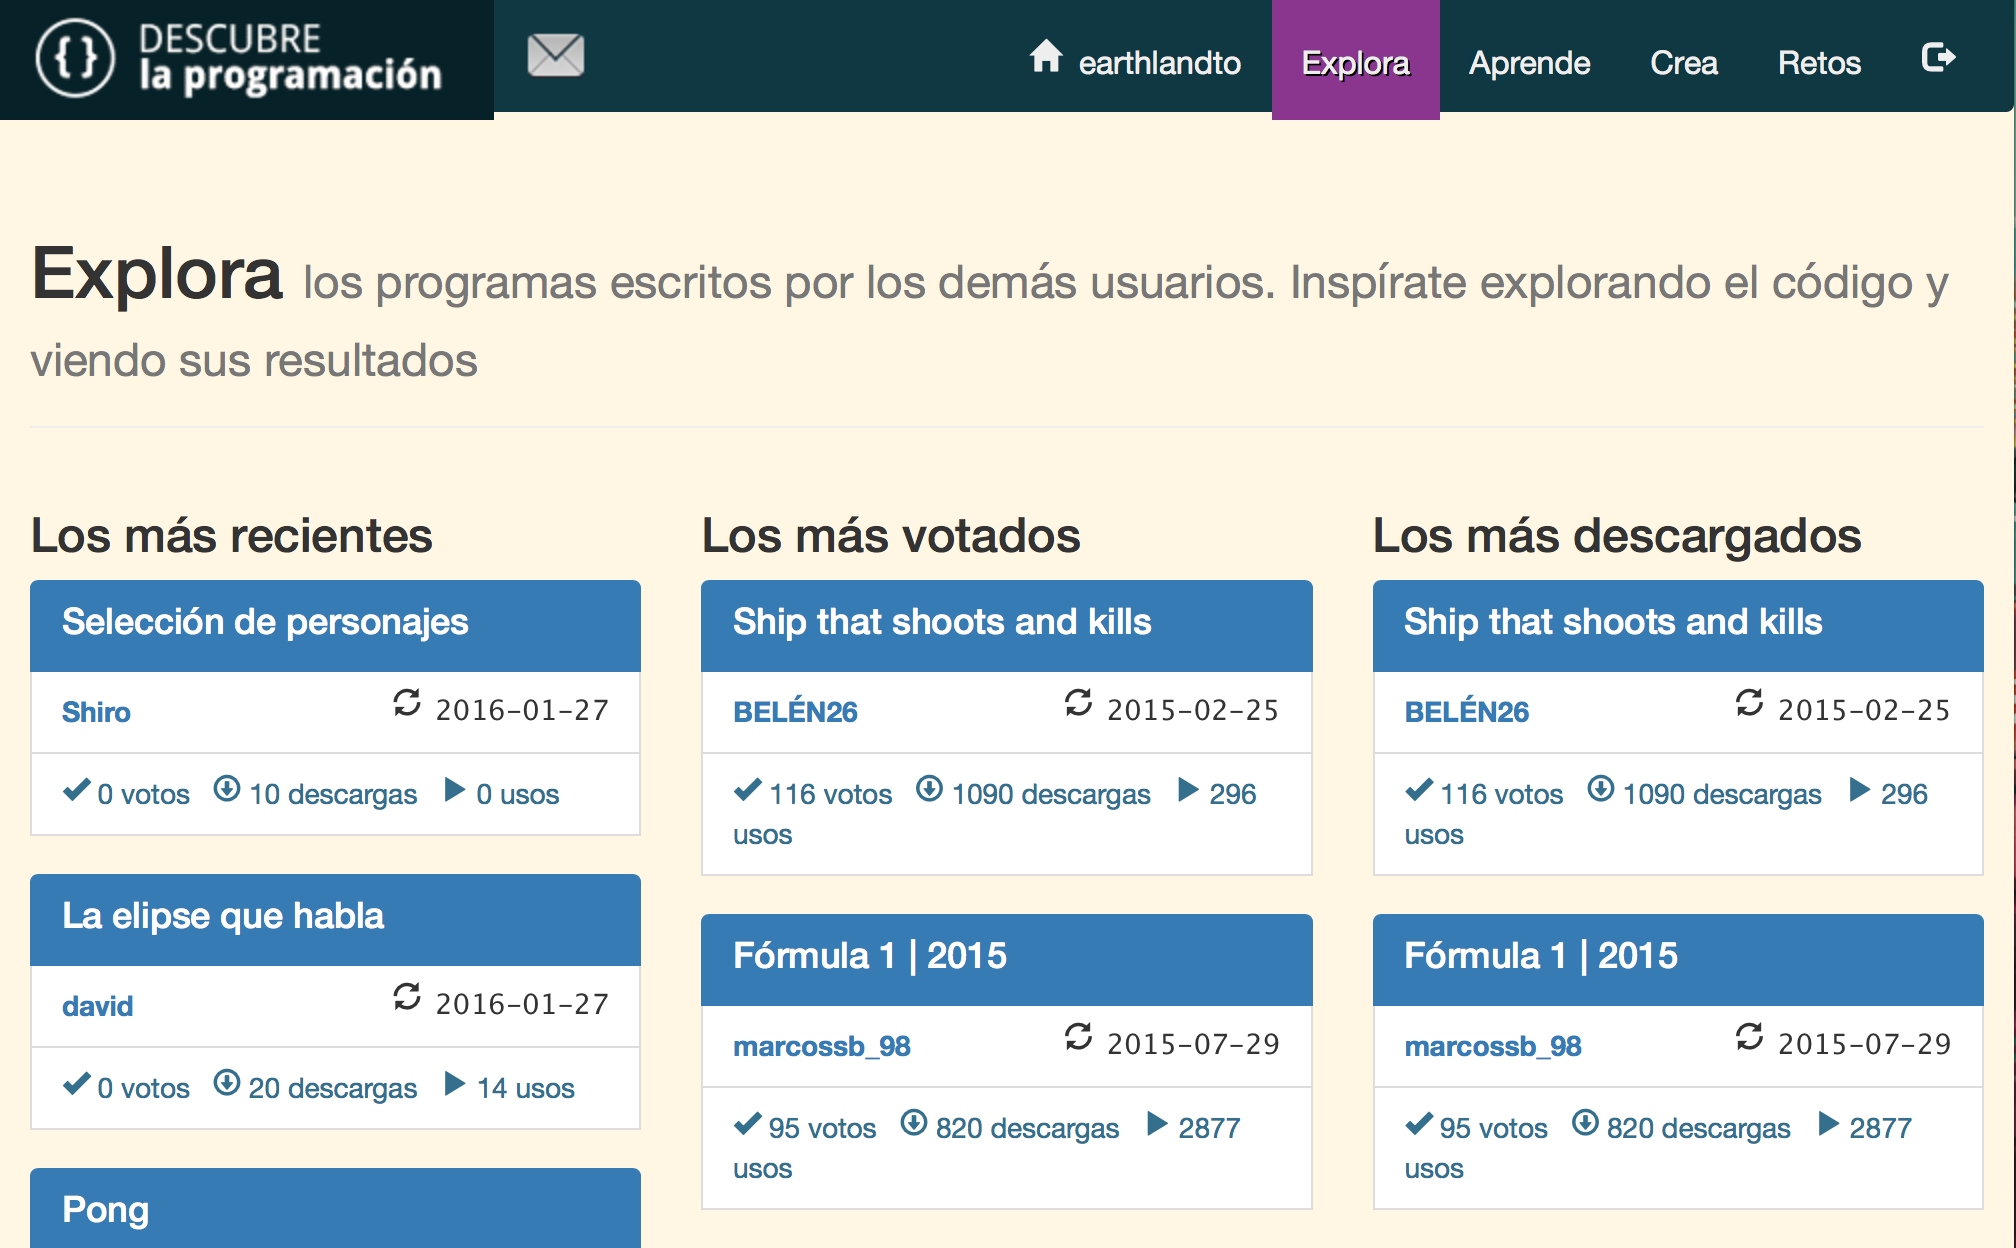
\includegraphics[width=0.5\textwidth]{images/descubre-explora.png}
% 				\caption{Sección \emph{Explora} del proyecto \Gls{descubre}. Obtenido de \cite{descubre}.}
% 				\label{fig:descubre-explora}
% 	\end{centering}
% \end{figure}
%
%
%
% \begin{figure}[!ht]
% 	\begin{centering}
% 		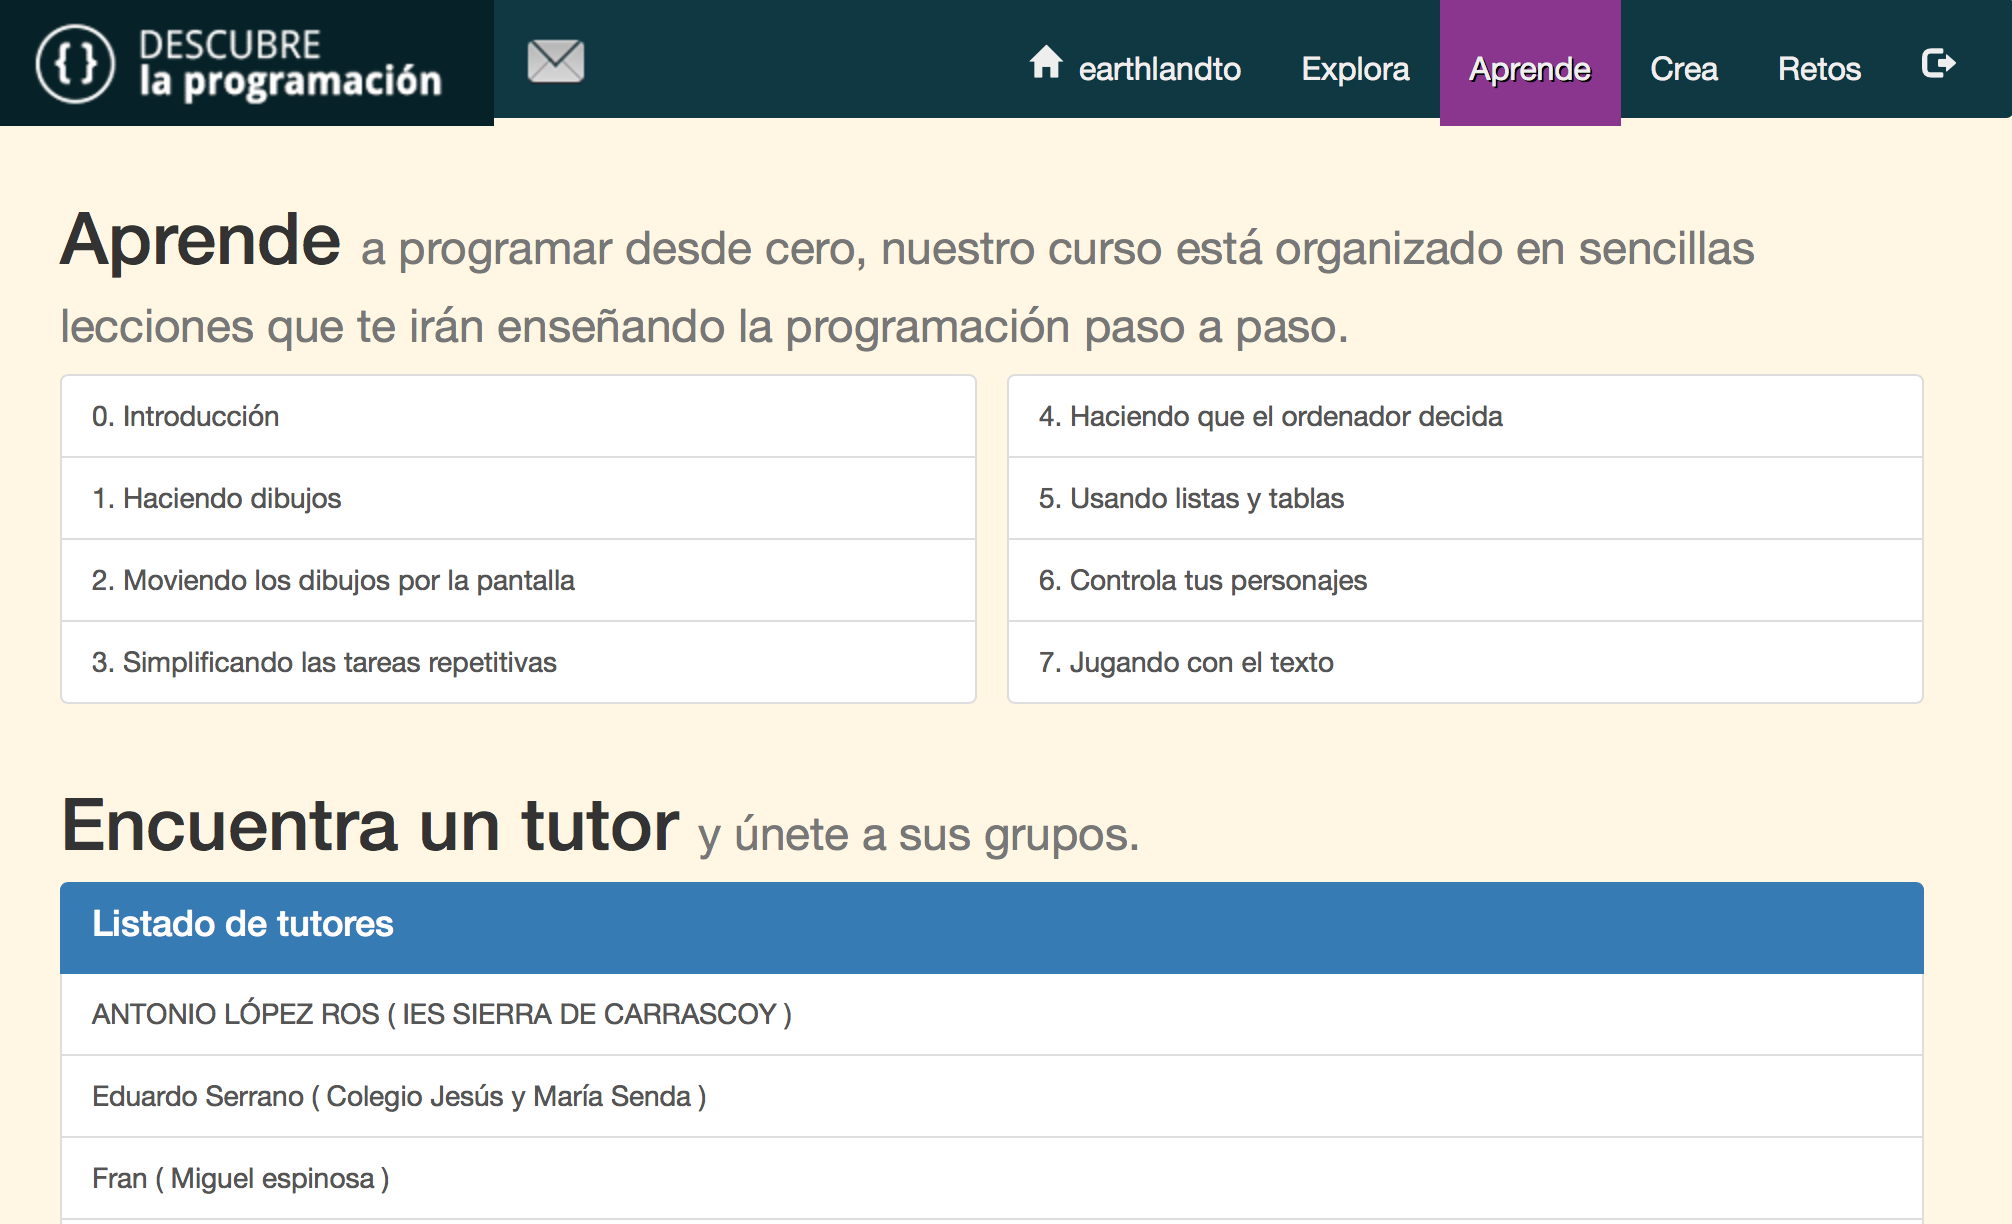
\includegraphics[width=0.5\textwidth]{images/descubre-aprende.png}
% 				\caption{Sección \emph{Aprende} del proyecto \Gls{descubre}. Obtenido de \cite{descubre}.}
% 				\label{fig:descubre-aprende}
% 	\end{centering}
% \end{figure}
%
%
% \begin{figure}[!ht]
% 	\begin{centering}
% 		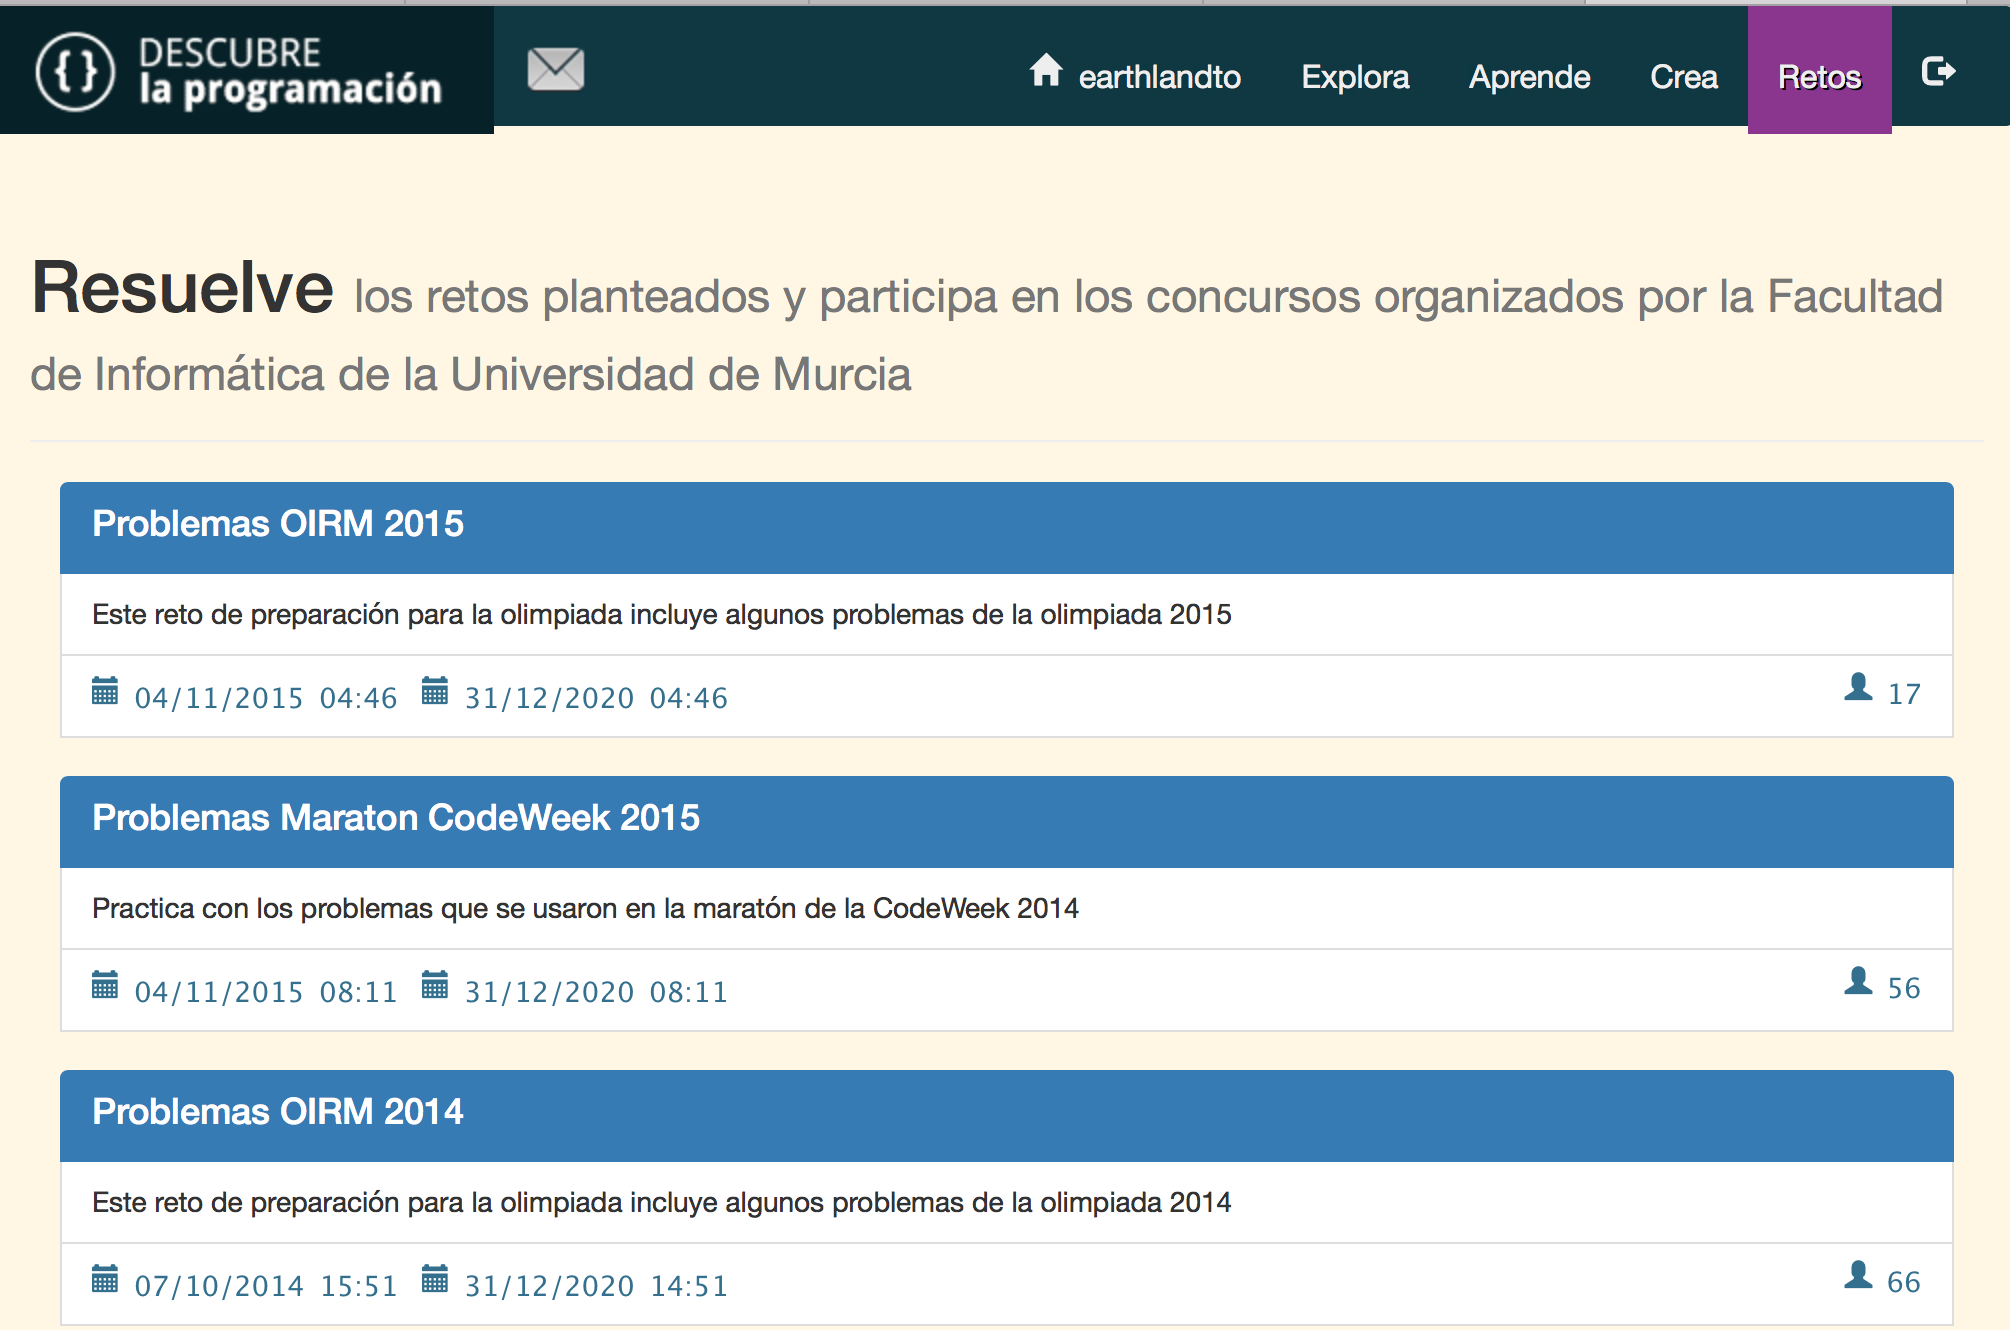
\includegraphics[width=0.5\textwidth]{images/descubre-retos.png}
% 				\caption{Sección \emph{Retos} del proyecto \Gls{descubre}. Obtenido de \cite{descubre}.}
% 				\label{fig:descubre-retos}
% 	\end{centering}
% \end{figure}
%
%
% \begin{figure}[!ht]
% 	\begin{centering}
% 		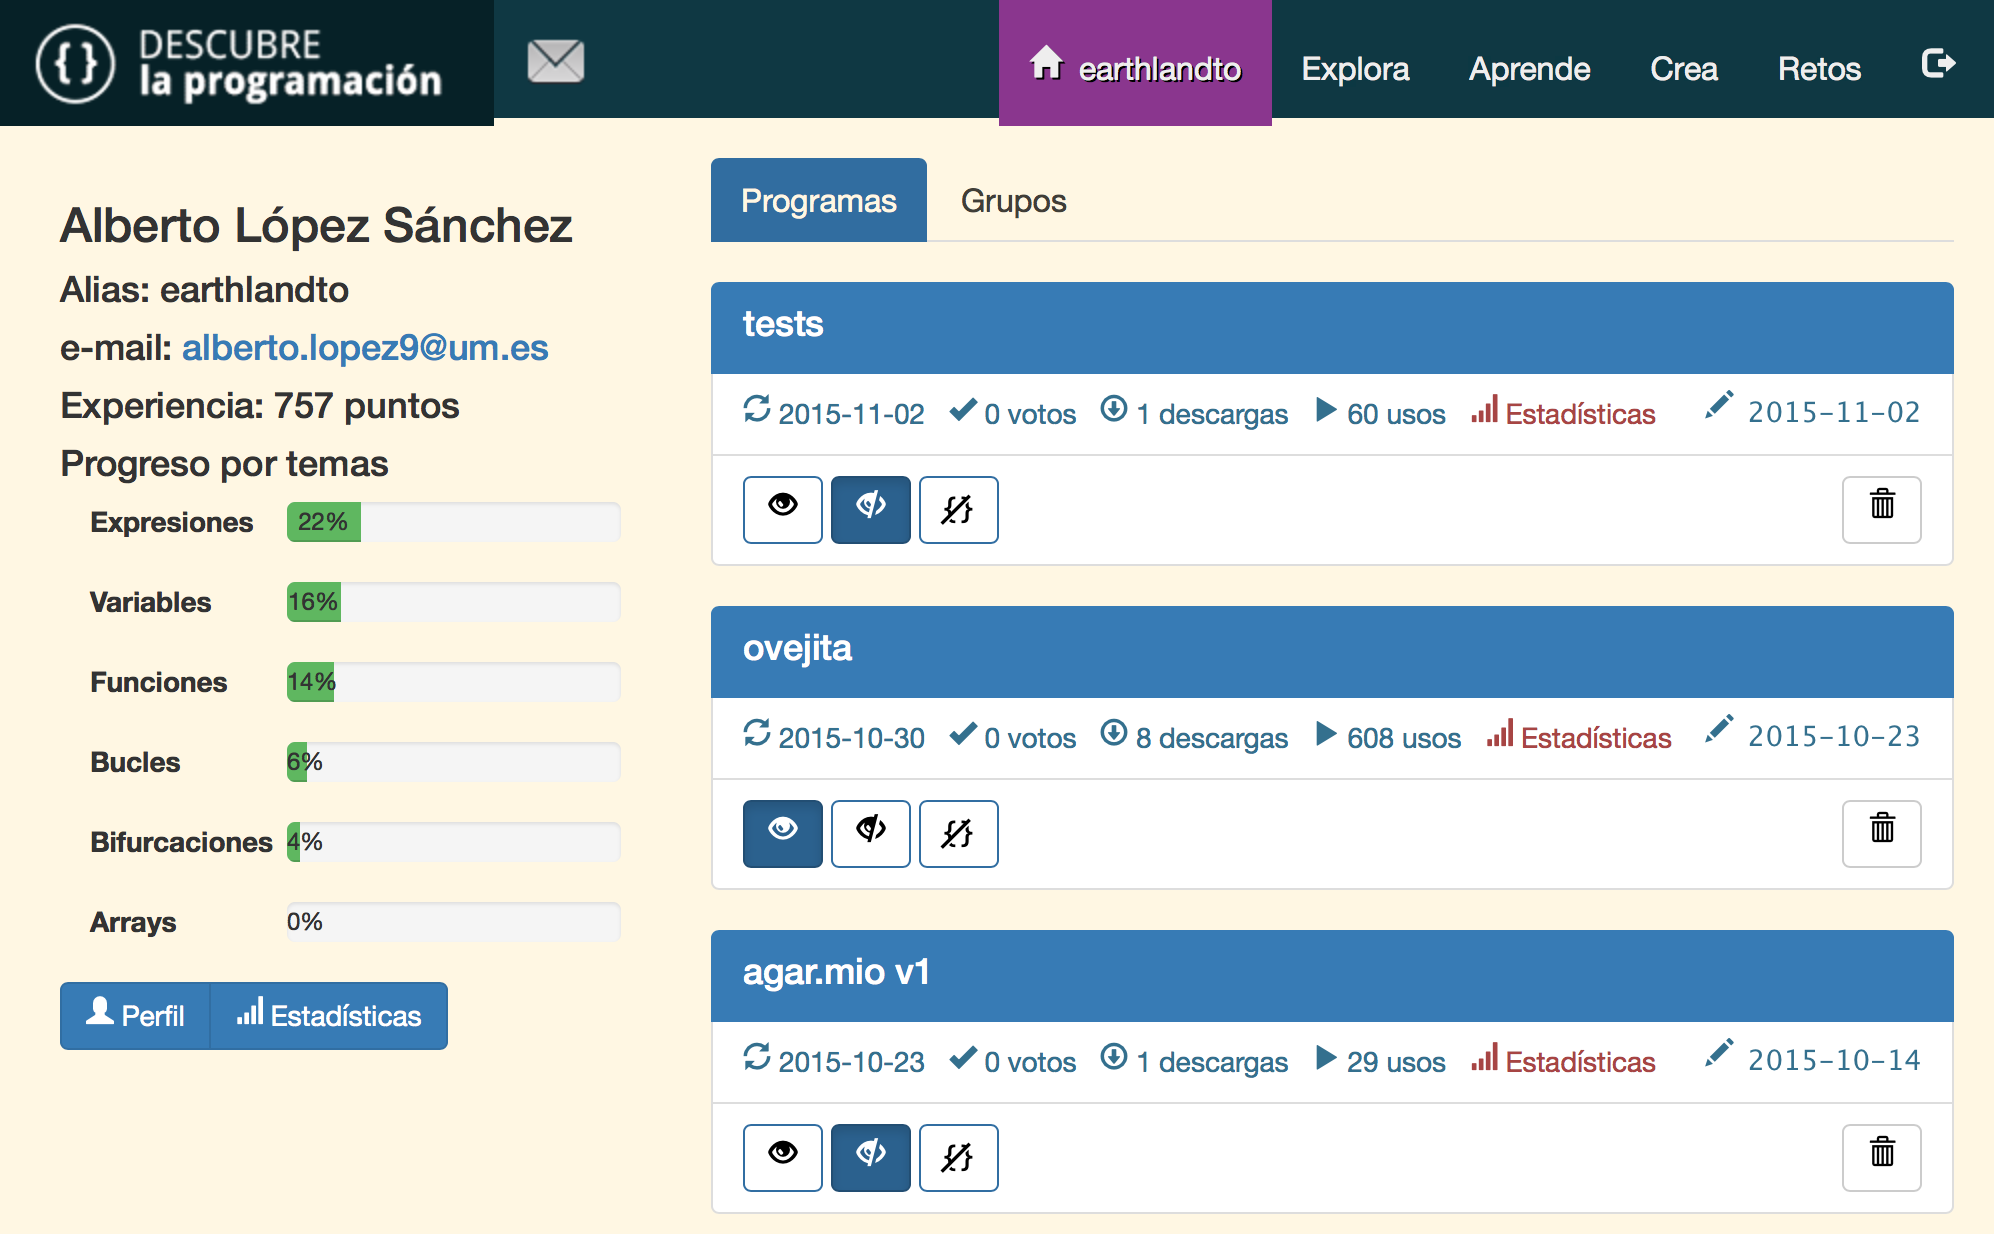
\includegraphics[width=0.5\textwidth]{images/descubre-profile.png}
% 				\caption{Vista del perfil de usuario del proyecto \Gls{descubre}. Obtenido de \cite{descubre}.}
% 				\label{fig:descubre-perfil}
% 	\end{centering}
% \end{figure}
%
%
% \begin{figure}[!ht]
% 	\begin{centering}
% 		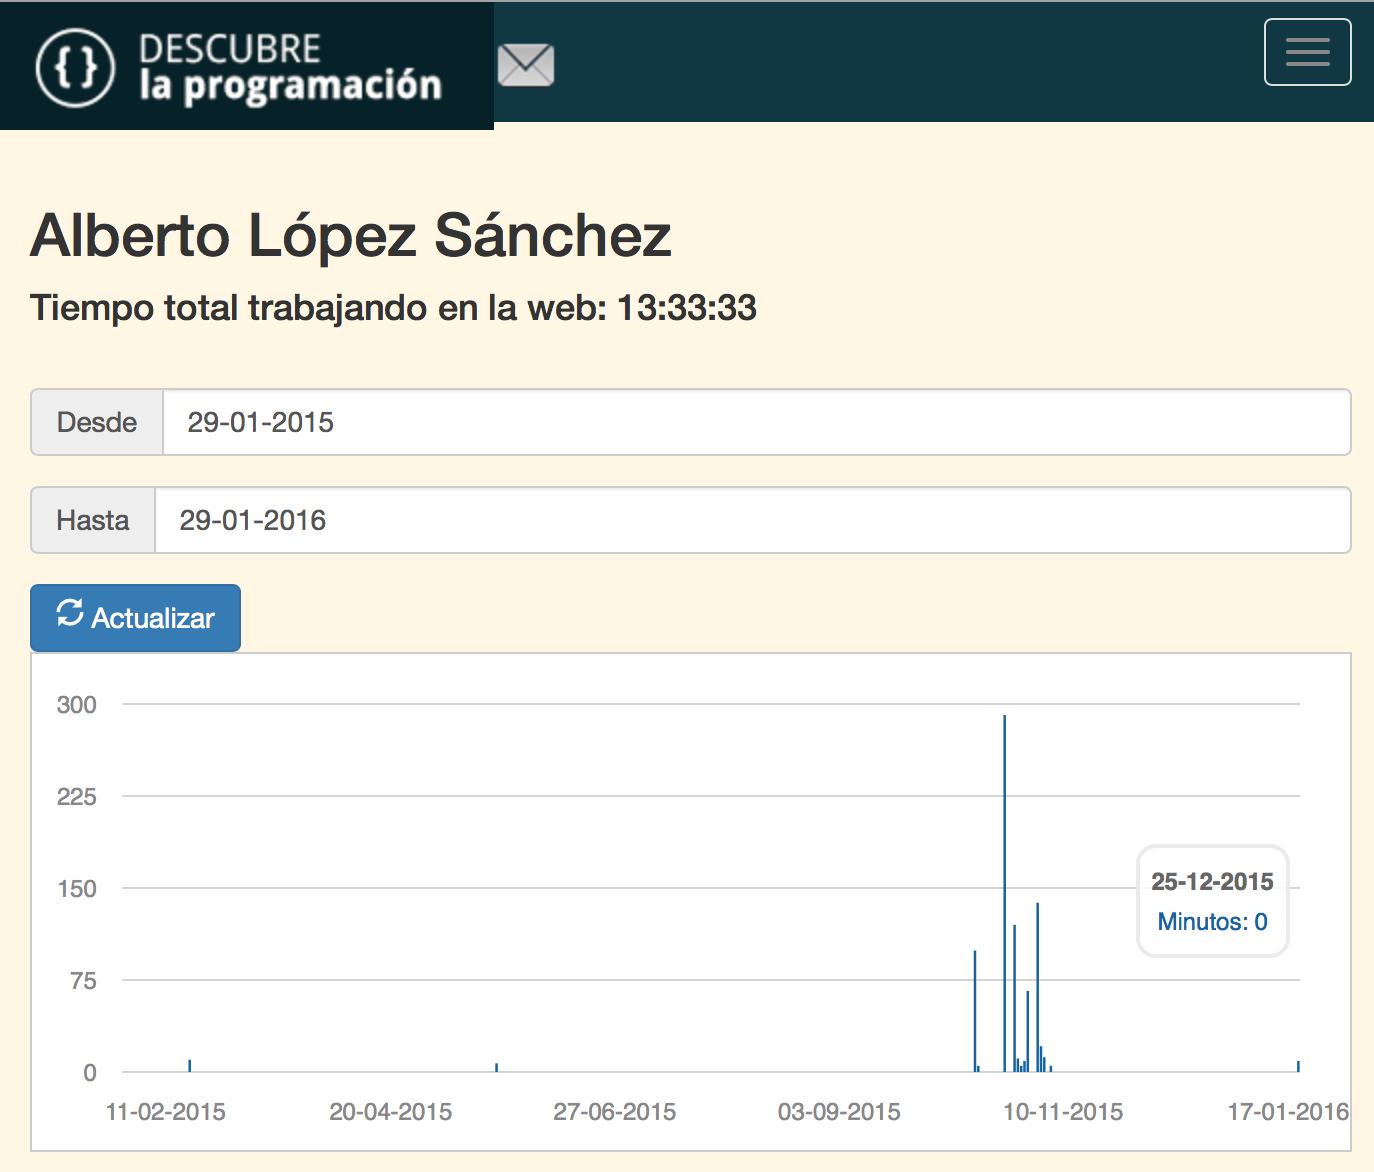
\includegraphics[width=0.5\textwidth]{images/descubre-statistics.png}
% 				\caption{Sección de estadísticas del usuario del proyecto \Gls{descubre}. Obtenido de \cite{descubre}.}
% 				\label{fig:descubre-estadisticas}
% 	\end{centering}
% \end{figure}


\begin{figure}[!ht]
	\begin{centering}
		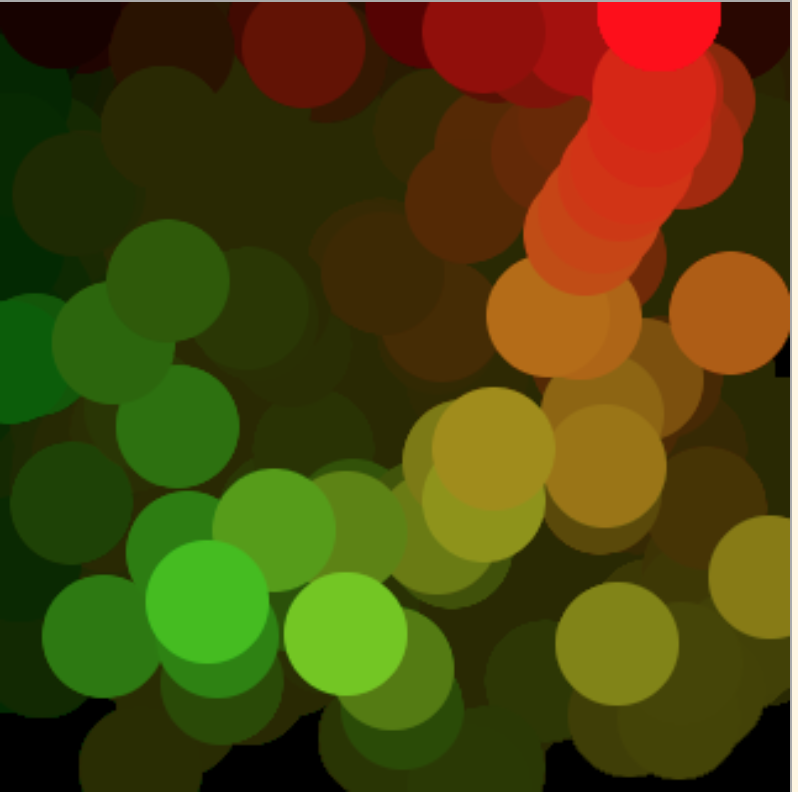
\includegraphics[width=0.5\textwidth]{images/salida-code-circulos-color-raton.png}
			\caption{Salida del programa escrito en iJava ejecutado por el código \ref{code:circulos-color-raton}.}
				\label{fig:salida-code-circulos-color-raton}
	\end{centering}
\end{figure}



\section{Motivación y enfoque de este proyecto}
\label{sec:motivacion}

Las nuevas tecnologías están haciendo que cada vez más gente de todas las edades se interese por la informática, y más concretamente por la programación. Poco a poco la informática deja de ser cosa de un grupo selecto de gente que entiende su funcionamiento. Como bien argumenta J. Wing en \cite{wing2006computational} y \cite{Wing3717}, se debería extender el pensamiento computacional en ambientes pre-universitarios y exponer a los alumnos al pensamiento y a los métodos computacionales.

Como ya hemos comentado anteriormente, existe un movimiento que pretende introducir la informática y la programación en las aulas puesto que se han demostrado los beneficios de enseñar a programar en una edad escolar temprana.

Es en este momento cuando se hace imprescindible tomar decisiones acertadas. Aprender a programar en edades pre-universitaria debe ser algo accesible a cualquier estudiante, independiente de su condición o los antecedentes del mismo. Igualmente, los conceptos de programación deben ser presentados de manera incremental, empezando por los más simples para luego ampliar a conceptos más complejos, como defiende L. Fernandez y otros en \cite{fernandez2002analisis}.

Este proyecto se enfocará desarrollando un simulador de robot de dos ruedas en el que los alumnos puedan programar su comportamiento. Se ofrece una librería de funciones para simplificar la interacción con el mismo y conseguir cierta funcionalidad extra que simplifique la tarea de comprensión y usabilidad del simulador.

El simulador se integrará en la plataforma Descubre la programación, mencionada en la sección \ref{sec:descubre}. Esto supone que el estudiante programará el comportamiento del robot simulado en iJava. El robot estará dentro de un circuito con distintos elementos con los que podrá interactuar. Asimismo, el robot dispondrá de una serie de sensores para poder recibir información del mundo que le rodea.

Al incluir el simulador como un módulo de Descubre, se pretende reforzar el esfuerzo por parte de sus creadores de hacer llegar la programación al mayor numero de estudiantes pre-universitarios posible, proponiendo una alternativa atractiva y que añade una componente más de entretenimiento a la actividad de programar. Por otra parte, permite que el alumno asimile conceptos de robótica de manera transparente. Al utilizar una plataforma web y de libre acceso, también se busca eliminar la barrera que puede suponer realizar una inversión en material electrónico como puede ocurrir con Arduino, Raspberry Pi o Lego.


Igualmente, los estudiantes que ya están usando la plataforma Descubre, podrán trabajar los conceptos de programación (bucles, condiciones, variables y funciones, entre otros) en un entorno diferente, renovando así su interés en otra actividad y aprender jugando.


%Esto permitirá ligar con la siguiente sección en la que se decide ampliar descubre añadiendo el simulador del robot. La justificación puede ser que de este modo se permite a quien no tiene recursos materiales para comprar el hardware o es ménos hábil con los aspectos mecánicos y electrónicos que también programe robots.


%% Último párrafo: explicar de que van las siguientes secciones.
En el capítulo \ref{estado-arte} se analizaran cuales son las alternativas que existen actualmente que trabajan en esta linea. En el capítulo \ref{diseno} se verá como se ha desarrollado la idea principal y que resultados se han obtenido. Por último, en el capítulo \ref{conslusiones} se analizarán los objetivos conseguidos y que ofrece mi propuesta en comparación a los proyectos actuales.



%%%%%%%%%%%%%%%%%%%%%%%%%%%%%%%%%%%%%%%%%%%%%%%%
% 2: Estado del arte
%%%%%%%%%%%%%%%%%%%%%%%%%%%%%%%%%%%%%%%%%%%%%%%%
\chapter{Estado del arte}\label{estado-arte}



A nivel global y desde hace varias décadas, existe una gran cantidad de proyectos con la única intención de enseñar, a alumnos de Educación Primaria, Secundaria y Bachillerato, diferentes aspectos de la informática como lo es la programación \cite{code-school,code-org,code-academy}, la robótica \cite{robomind-web,moway} e incluso electrónica (con \Gls{arduino}\cite{arduino}, Raspberry Pi\cite{raspberry-pi} o Lego Mindstorm\cite{lego-mindstorm-programar}).
La mayoría de estos proyectos promueven una enseñanza independiente y autodidacta bajo un entorno on-line y gratuito. De esta manera, el alumno puede aprender a su propio ritmo y desde cualquier parte del mundo.

En las siguientes secciones se hablará del \Gls{logo}\cite{logo} y el proyecto \Gls{turtle}\cite{logo-turtle}, un proyecto que lleva décadas activo, con la principal finalidad de enseñar programación y matemáticas a niños. También se estudiarán los diferentes proyectos que existen actualmente y que promueven una enseñanza a niños en entornos web. Por último, se analizarán los diferentes proyectos que enseñan programación jugando y que utilizan robots y/o simuladores.


\section{Logo y el robot Turtle}
\label{sec:Logo}

El lenguaje Logo, desarrollado a finales de la decada de los 60 y basado en \Gls{lisp}, fue diseñado como una herramienta de aprendizaje a niños. Todas sus características -interactividad, modularidad, extensibilidad, flexibilidad en los tipos de datos- persiguen esta meta. El lenguaje Logo fue uno de los primeros proyectos en emprender la difícil tarea de enseñar a programar a niños de Primaria.


Como se explica en la página oficial del proyecto Logo\cite{logo}, durante la década de los 70, en el \acrfull{MIT} y diferentes centros de investigación europeos, se llevaron a cabo investigaciones sobre el uso del \Gls{logo} en pequeños grupos de alumnos de Educación Primaria.

A pesar de los diversos estudios que se han realizado a lo largo de los años, no se han conseguido obtener unos resultados claros sobre la posible ventaja de enseñar a programar a niños de Primaria y Secundaria con Logo. En \cite{feurzeig1969programming}, Feurzeig y otros consiguen una leve mejoría en la nota obtenida en el Test de Habilidades Básicas de Iowa (Iowa Test of Basic Skills, o ITBS)\footnote{El Iowa Test of Basic Skills (ITBS), es un test que se realiza anualmente siguiendo una serie de estándars a nivel de estado para medir el rendimiento académico de los alumnos en materias como: vocabulario, ortografía, algebra, conceptos aritméticos y comprensión de tablas y gráficos, entre otros.}. En la tabla \ref{tab:logo-itbs} se puede ver como la nota global del grupo que aprende a programar (denominado \emph{computer}) es de 114 puntos más que el curso anterior, mientras que la obtención del grupo de control es solo de 6 puntos. Aún así, se puede ver como la nota del grupo de control sigue siendo mayor que la del grupo \emph{computer}. Ante éste hecho, Feurzeig concluye que el grupo de control no representaba muy bien al grupo \emph{computer} y que, por tanto, la comparación perdía validez.
Más tarde, Pea y Kurland en \cite{pea1984logo} concluyen que, tras el estudio en dos cursos separados de alumnos, aprender a programar no conseguía mostrar ningún beneficio claro en el rendimiento de los alumnos en comparación al grupo de control.
Poco más tarde, Moss \cite{moss1985creating} obtiene evidencias de la relación en el aprendizaje de Logo con el desarrollo de conceptos primitivos que más adelante se enlazarían con la álgebra básica.


\begin{table}[!ht]
	\begin{centering}
		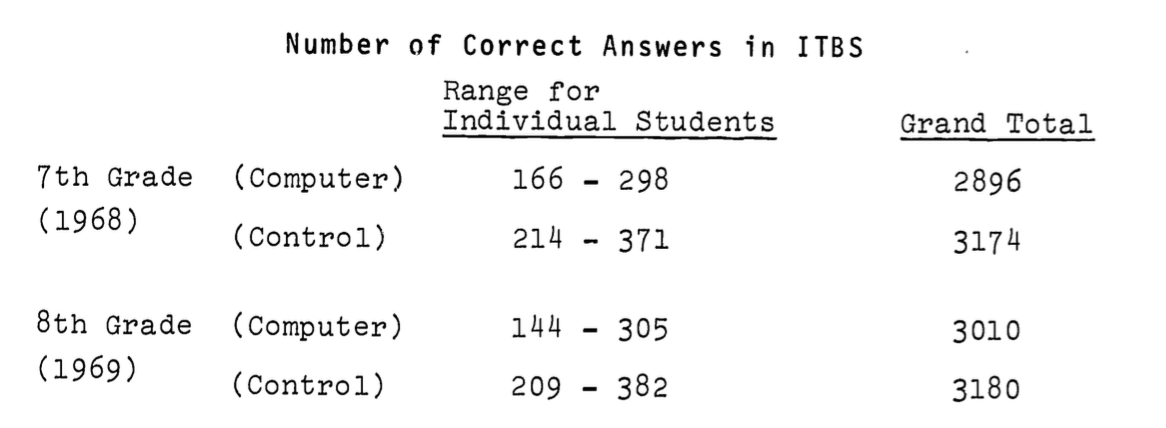
\includegraphics[width=0.8\textwidth]{images/logo-itbs.png}
			\caption{Tabla que muestra los resultados obtenidos en el ITBS por los alumnos que aprendierona programar (denominado \emph{computer}) y el grupo de control. Obtenido de \cite[p.251]{feurzeig1969programming}.}
				\label{tab:logo-itbs}
	\end{centering}
\end{table}


En el Apéndice \ref{anexo:logo-lenguaje} se hace un breve estudio del lenguaje Logo y las principales características que posee el lenguaje.



\subsection{Turtle de Logo}
\label{sec:turtle}

El proyecto \emph{Turtle} es el proyecto más popular del lenguaje Logo. Nació como una criatura robótica, arreglada para que pareciera una tortuga, que se movía por el suelo con un rotulador atado que pintaba el suelo. Más tarde evolucionó a una imagen de una tortuga que se movía por la pantalla pintando según se desplazaba. Turtle se utiliza ampliamente desde hace décadas para enseñar a programar a niños de Primaria y Secundaria conceptos de programación, pero también de matemáticas y geometría\cite{abelson1980disessa,brown1995101}.

A pesar de su larga vida, el proyecto Turtle ha sabido mantenerse vivo y se ha modernizado en proyectos más recientes como Turtle Academy \cite{turtle-academy} o Curly Logo \cite{curly-logo}.

En el apéndice {anexo:logo-turtle-lenguaje} se puede consultar información sobre cual es el funcionamiento de Turtle.


\section{Scratch}
\label{sec:scratch}


Scratch\cite{scratch} es un proyecto creado en el seno del Lifelong Kindergarten Group en el MIT Media Lab, \acrfull{MIT}. Permite programar juegos interactivos, animaciones y programas de todo tipo en un entorno web. Todo esto apoyado por una gran comunidad de usuarios y profesores que forman una enorme red social de más de 9.5 millones de usuarios registrados y casi 13 millones de proyectos compartidos actualmente\footnote{En la página oficial de Scratch se pueden obtener las estadísticas de uso y participación (\url{https://scratch.mit.edu/statistics/}).}.

Scratch está orientado a enseñar a programar a niños de Primaria y Secundaria y como se puede apreciar en la figura \ref{fig:scratch-edad} la mayoría de usuarios de Scratch cumplen dicho perfil, la edad está en torno a los 12 y 15 años.

\begin{figure}[!ht]
	\begin{centering}
		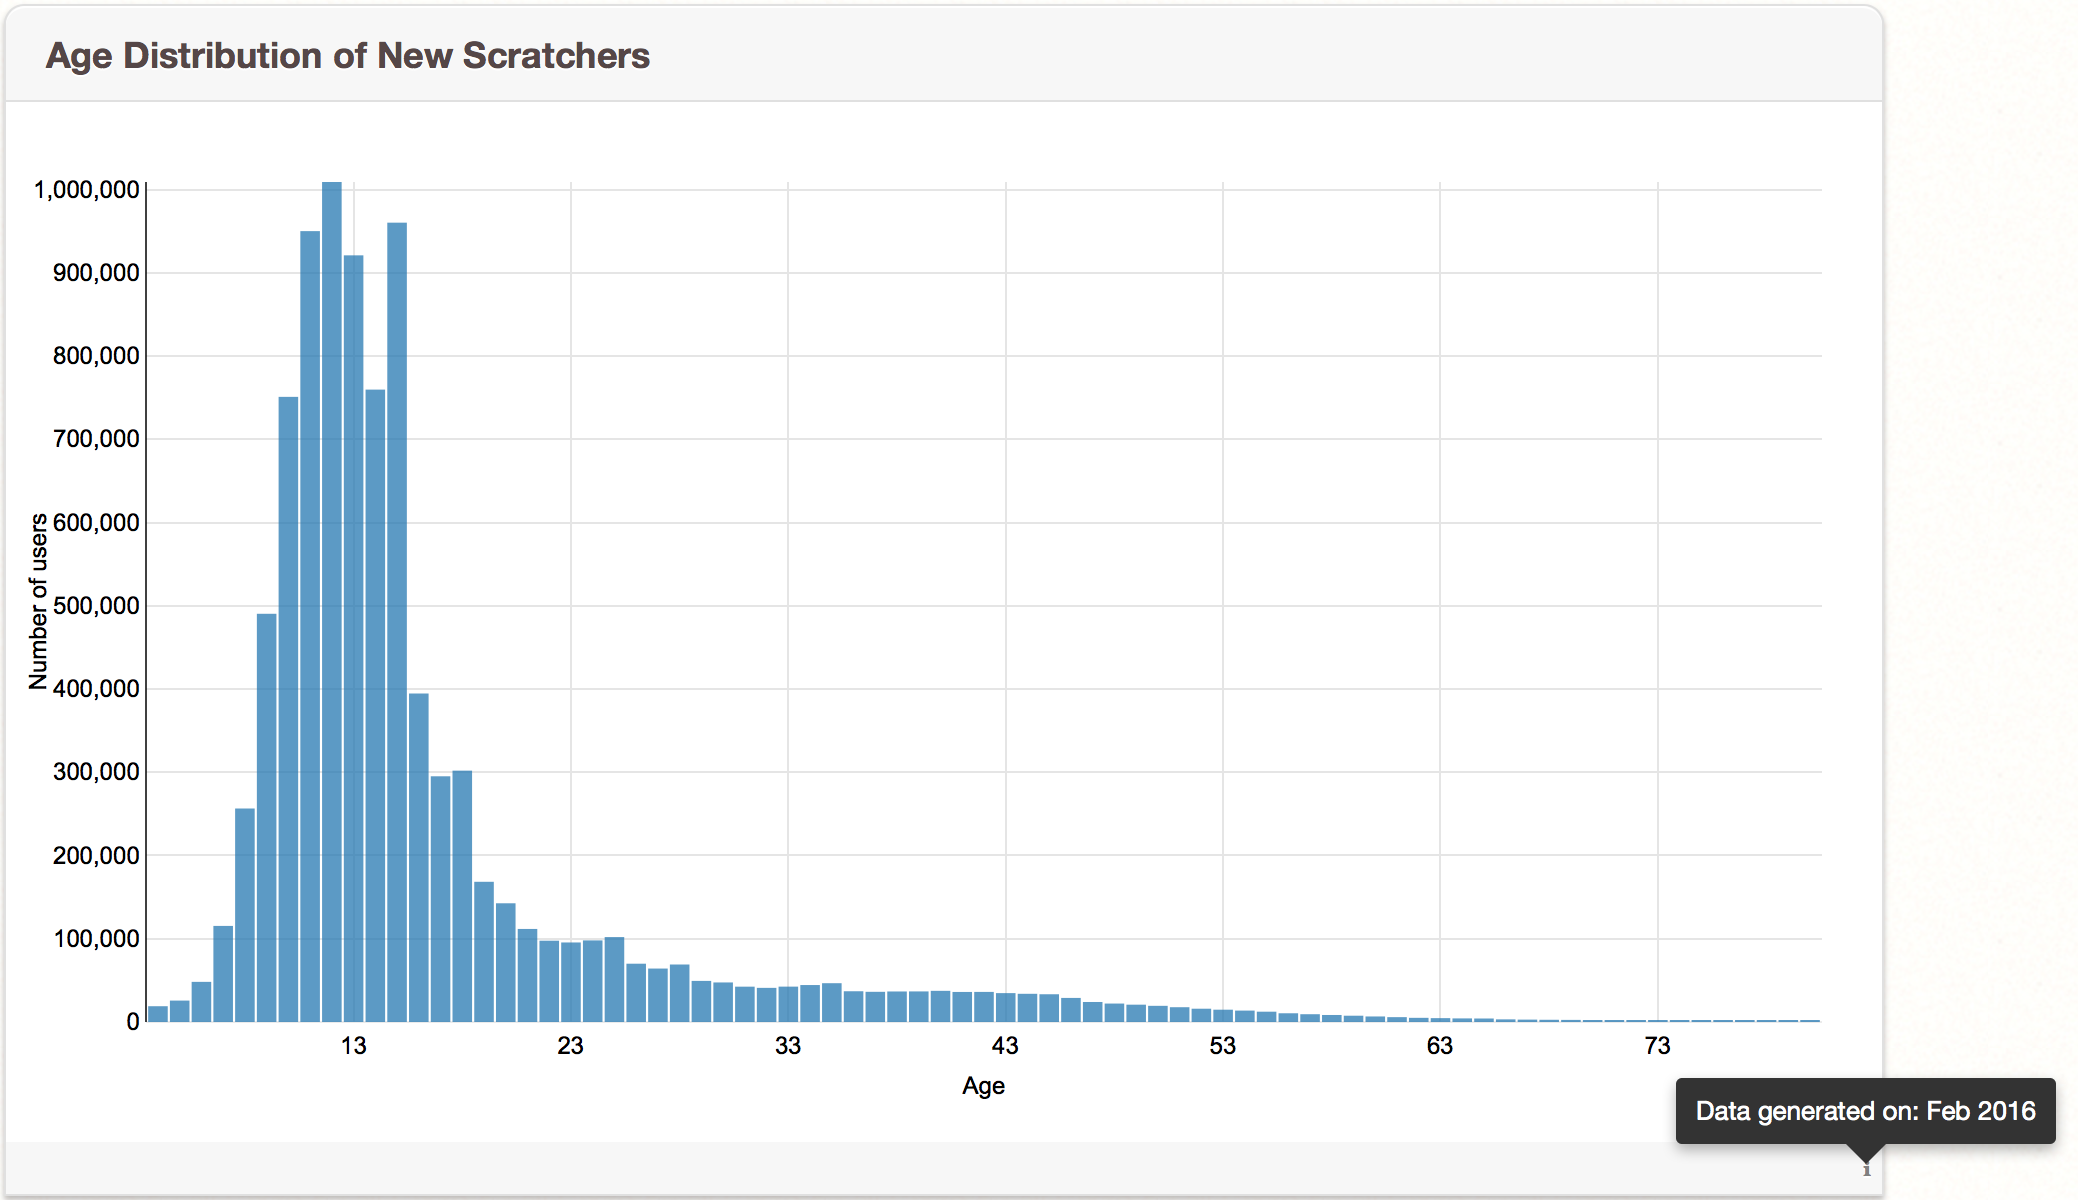
\includegraphics[width=0.8\textwidth]{images/scratch-edad.png}
			\caption{Gráfico de edad de los usuarios de Scratch. Obtenido de \url{https://scratch.mit.edu/statistics/}.}
				\label{fig:scratch-edad}
	\end{centering}
\end{figure}


La idea básica para programar con Scratch es la de crear el flujo del programa mediante la unión de bloques que representan las diferentes funcionalidades del lenguaje (crear o modificar variables, bucles, condiciones, funciones de librería, etc). Existen dependencias entre la forma de los bloques, de esta manera, solo unos bloques \emph{encajaran} con los que tengan una forma compatible. De esta manera, se consigue una relación visual y directa por parte del programador entre los bloques que puedes unir, y sobretodo, de lo que no puedes hacer.

Para saber más sobre el funcionamiento de Scratch y como se programa con esta herramienta se puede consultar el apéndice \ref{anexo:scratch-funcionamiento}.

Como conclusión, Scratch es un entorno completo y autosuficiente con una gran y compleja funcionalidad que permite a niños y mayores realizar aplicaciones sin necesidad de saber programar pero aprendiendo conceptos básicos como la repetición, el control de instrucciones y como llevar a cabo una animación. 



\section{Aprendiendo con robots}
\label{sec:aprendiendo-robots}


En secciones anteriores se han analizado dos formas de aprender a programar. Logo, junto a Turtle, fue el primer lenguaje de programación que se creó para enseñar a programar a niños de Primaria y Secundaria. Por otra parte, Scratch es actualmente un gran promotor del \emph{Computational Thinking} con una cantidad considerable de usuarios activos.

No obstante, existen otros enfoques para enseñar programación y desarrollar el pensamiento computacional. La robótica es una opción muy extendida y que atrae a partes iguales a alumnos y docentes. En las siguientes secciones se estudiaran diferentes alternativas que utilizar tanto simuladores como robots reales.


\subsection{Lego Mindstorm NXT/EV3}
\label{sec:lego-nxt-ec3}

Como se ha mencionado en la sección \ref{sec:electronica-robotica}, el proyecto Lego Mindstorm\cite{lego-mindstorm} está orientado a enseñar robótica a estudiantes de Primaria y Secundaria. Lego proporciona dos kits para crear tu propio robot: NXT y EV3. Lego Mindstorm NXT\footnote{Actualmente, Lego Mindstorm NXT tiene soporte por parte de Lego hasta finales del año 2015.} fue lanzado en 2006, y su siguiente versión, Lego Mindstorm EV3, salió al público en 2013. Tanto la versión NXT como EV3 son ampliamente utilizadas y existen una gran cantidad de competiciones que fomentan su uso.

Cada kit está compuesto por elementos Software para poder programar el comportamiento del robot y elementos Hardware como sensores, accesorios, piezas de lego y el \emph{Brick} (ladrillo). El \emph{Brick} es un aparato con el que se pueden programar comportamientos básicos a las piezas conectadas al mismo, pero principalmente es el cerebro de todo el robot. Las piezas son mayormente compatibles entre los dos sistemas, la diferencia radica en el \emph{Brick}. 

En concreto, EV3 viene acompañado del \emph{Lego Mindstorm EV3 Home Edition Software} y su \emph{brick}, el \emph{Brick P EV3}. De esta manera se puede programar instrucciones al robot con bloques (o iconos) que recuerdan a Scratch. Los bloques representan diferentes funciones del lenguaje y el programador debe conectar dichos bloques para crear el flujo de ejecución del programa. Lego también ofrece \emph{EV3 Programmer}, una versión gratuita y simplificada (con menos funcionalidad y bloques) para programar los robots de Lego.

Los bloques se dividen en: bloques de acción, bloques de flujo, bloques de sensores, bloques de operación de datos y bloques avanzados. 
Los bloques de acción permiten controlar la rotación de los motores y las luces del \emph{Brick P EV3}. Los bloques de flujo definen cual será el flujo del programa, cuyo inicio se define con el \emph{bloque de inicio}. Los bloques de sensores, entre otras funciones, controlan los sensores táctiles y de color conectados al \emph{brick}. Los sensores de operación de datos permiten definir variables, realizar cálculos matemáticos u obtener valores aleatorios. Por último, los bloques avanzados permiten administrar ficheros o establecer conexiones Bluetooth.

Por otra parte, existen muchas aplicaciones de terceros no oficiales que permiten utilizar lenguajes de programación de alto nivel para controlar el robot, como pueden ser Python, Lua, .Net, C/C++, Java o Robomind (del cual hablaremos en la sección \ref{sec:robomind}).


\subsection{Moway}
\label{sec:moway}


El robot Moway\cite{moway} es un robot desarrollado como herramienta educativa. Moway se compone por un conjunto de sensores y actuadores que le permiten recibir información del mundo real y reaccionar a la misma según las instrucciones que se le hayan proporcionado.

Los actuadores de los que dispone el robot Moway son: dos ruedas, luces LEDs y un altavoz. Por otra parte, los sensores de los que dispone Moway son:
 
\begin{itemize}
	\item Un sensor de luz que le permite detectar el nivel de luz ambiente. 
	\item 2 sensores de linea, mirando hacia el suelo, que detectan diferencias de color.
	\item 4 sensores de obstáculos en la parte frontal del robot que detectan la distancia a los mismos.
	\item Un micrófono para detectar el nivel de ruido.
	\item Un sensor de temperatura. 
	\item Un acelerómetro que detecta inclinación y fuerzas.
\end{itemize}

La aplicación gratuita Moway World permite crear diagramas de flujo para programar el comportamiento del robot, con funciones para activar y controlar los diferentes actuadores del robot Moway en función de la información obtenida por los sensores. También permite programar su funcionamiento con Scratch, el cual se ha analizado en la sección \ref{sec:scratch}. 

Moway tiene varios módulos que pueden ser añadidos para ampliar su funcionalidad o manejo, como son: módulos de radiofrecuencia, placas Raspberry Pi, tarjetas wifi o una cámara para captar imágenes en tiempo real. También se ofrece una alternativa a Moway de código abierto, llamada Mowayduino. Mowayduino está basado en Arduino y tiene toda la funcionalidad y potencia que ofrece Arduino. Los kits que se disponen inicialmente para Mowaiduino son los mismos que para Moway. Para programar un Mowayduino se proporciona el entorno de programación oficial de Arduino.


Un uso común de Moway es como robot \emph{sigue-lineas}. Los sensores de linea de los que dispone proporcionan información para poder conocer el estado del robot con respecto a una linea, es decir, si está sobre una linea o no. Al tener 2 sensores, puede conocer si se está saliendo de la linea (quizás porque esta realiza una curva) y en la dirección en la que esto ocurre. Por ejemplo, si el sensor derecho deja de detectar la linea, quiere decir que: o la linea está realizando una curva hacia la izquierda o que el robot Moway está moviéndose hacia la derecha fuera de la linea (lo cual ocurre en ambos casos, si se analiza la situación desde el punto de vista de la linea). Por tanto, al estar saliéndose de la linea por la derecha, el robot Moway tendrá que moverse hacia la izquierda para mantenerse dentro del la misma. 


En general, Moway ofrece un robot para programarlo y configurarlo junto a un entorno de programación, como puede ser Scratch. Es un buen inicio en la robótica pero su software privativo deja las opciones de ampliación y de creación de complementos y terceras partes un poco limitadas.

Moway, junto a Robomind, será uno de los pilares en los que se basará el simulador que se desarrollará, en especial la parte que tiene que ver con las características del simulador.



\subsection{Karel the Robot}
\label{sec:karel-the-robot}


Karel\footnote{El nombre de Karel the robot es nombrado en honor a Karel Čapek, un escritor checo que introdujo el término \emph{robot} por primera vez.} es un lenguaje de programación creado por R. Pattis en su libro \emph{Karel the robot: A gentle introduction to the Art of Programming} (El robot Karel: Una introducción gentil al arte de programar) en 1981\cite{pattis1981karel}. En el, Pattis enseña conceptos de programación siguiendo una metodogía \emph{Early bird}\cite{early-bird}, que consiste en enseñar primero los conceptos más importantes.

Karel se mueve en un escenario discreto con celdas y con el que se puede interactuar. Las órdenes básicas del robot Karel son: \texttt{move} para avanzar una posición en la dirección que está mirando; \texttt{turnLeft} para girar 90º en sentido contrario a las agujas del reloj; \texttt{putBeeper} y \texttt{pickBeeper} para depositar o recoger, respectivamente, un \emph{beeper} (localizador) en la posición en la que se encuentra Karel; y por último, \texttt{turnoff}, para apagarse a si mismo y finalizar la ejecución del programa.

Adicionalmente, Karel también proporciona instrucciones para comprobar si hay obstáculos o un \emph{beeper} en la posición que se encuentra. Toda esta funcionalidad viene acompañada de instrucciones de control, bucles y operaciones aritméticas.




\subsection{Robomind}
\label{sec:robomind}


Robomind Academy\cite{robomind-web} es una plataforma que busca potenciar y extender el \emph{Computational Thinking} entre alumnos de Educación Primaria y Secundaria. Sus creadores opinan\footnote{En la sección \emph{Visión} de la página web oficial de Robomind Academy se puede ver cuales son los principios y metas detrás del proyecto (\url{https://www.robomindacademy.com/go/robomind/about#vision}). Consultado el 2 de febrero de 2016.} que la informática debería tener el mismo estatus que las matemáticas o la lengua, algo esencial en la formación del estudiante. Argumentan que, a través del \emph{Computational Thinking} se podrán realizar avances en el cuidado de la salud o la industria, algo totalmente necesario en pleno Siglo XXI. 


Actualmente, Robomind ofrece un entorno de programación multiplataforma: aplicación de escritorio, entorno web y aplicación para Tablet. En la figura \ref{fig:robomind-entorno} podemos ver un ejemplo de como es el entorno de programación que propone Robomind.


\begin{figure}[!ht]
	\begin{centering}
		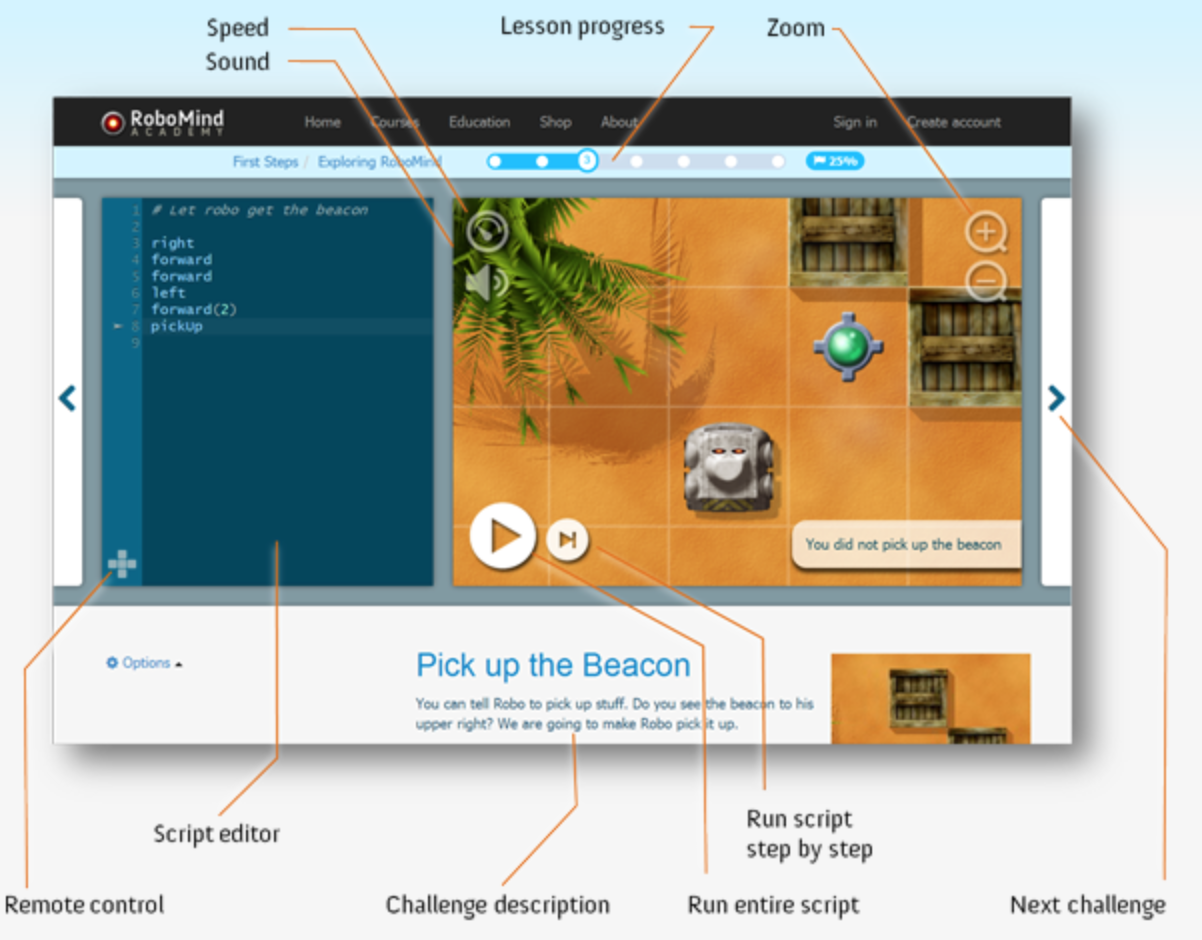
\includegraphics[width=0.8\textwidth]{images/robomind-entorno.png}
			\caption{Entorno de programación en Robomind Academy. Obtenido de \cite{robomind-web}.}
				\label{fig:robomind-entorno}
	\end{centering}
\end{figure}


El proyecto en sí está orientado a que profesores y alumnos trabajen conjuntamente en desarrollar las actividades, permitiendo que los profesores puedan realizar un seguimiento del avance y trabajo de los alumnos a cargo. También permite que los alumnos puedan registrarse independientemente y aprender a su propio ritmo. Los cursos están divididos entre alumnos de Educación Primaria y Secundaria. 

Las soluciones antes mencionadas son de pago. Dependiendo de si eres profesor o estudiante y de si quieres (o no) utilizar la versión de escritorio, se ofrecen distintos planes de compra. 
A parte, Robomind ofrece planes gratuitos para alumnos con características más limitadas o una cantidad inferior de cursos. Adicionalmente, Robomind participa en el proyecto \emph{La Hora del Código}\cite{hour-of-code}, ofreciendo una introducción a Robomind completamente gratuita. Una de sus funciones más interesantes es la de poder traducir el código escrito en Robomind para poder utilizarlo con tu propio Lego Mindstorm\footnote{Ya se ha hablado de Lego Mindstorm en la sección \ref{sec:lego-nxt-ec3}. Para más información sobre Lego Mindstorm NXT se puede acudir a \cite{lego-mindstorm}.}.

Por último, tanto la interfaz, la página web, la aplicación o los tutoriales está completamente en inglés, ofreciendo una cierta barrera de entrada a todo aquel interesado que no sea angloparlante. 

{\color{blue}
Para ampliar información de como se programa Robomind, se puede consultar el apéndice \ref{anexo:programacion-robomind}.

Como se puede ver, Robomind está formado por elementos de \emph{Karel the robot}, como lo es el movimiento en un escenario discreto y la forma de interactuar con el entorno, y por \emph{Turtle} de Logo y su capacidad de dejar un rastro por donde va pasando.
}


\section{Aprendizaje Online}
\label{sec:aprendiendo-online}

En la sección anterior se han analizado diferentes alternativas para aprender a través de la robótica. Algunas de estas alternativas tienen una gran componente Hardware, como puede ser Lego Minstorm. Por otra parte, Robomind, como simulador de un robot, permite al alumno iniciarse en la robótica sin necesidad  de un robot. 

Aunque es una práctica bastante utilizada, usar un robot no es la única alternativa para aprender a programar. Usar un entorno online para enseñar a programar es una alternativa que ha obtenido notable popularidad últimamente. Como se vio en la sección \ref{sec:scratch}, Scratch es un gran exponente del \emph{Computational Thinking} que utiliza un entorno principalmente online para que niños de todo el mundo aprenda a programar. Aunque éste no es el único proyecto que existe en esta linea. CodeHS y CodeSchool son algunos de los proyectos con más repercusión que buscan extender la cultura del \emph{Computational Thinking}, especialmente ente niños. En las siguientes secciones se estudiaran estas alternativas.

\subsection{CodeHS}
\label{sec:CodeHS}


Otro proyecto muy extendido que promueve el \emph{Computational Thinking} es CodeHS. CodeHS es una plataforma online con la que personas de todas las edades pueden aprender informática. Tienen cursos de introducción a la informática, programar con diferentes lenguajes, bases de datos, e incluso una versión modernizada de Karel the robot, el cual se ha analizado en la sección \ref{sec:karel-the-robot}.

CodeHS ofrece muchas opciones de aprendizaje independiente, incluso con tutores personalizados para resolver dudas de los usuarios, está especialmente dirigido a enseñar programación en colegios e institutos. Ofrece planes de pago para implantar la plataforma en las clases o herramientas de seguimiento y evaluación para que el profesor pueda supervisar el rendimiento de los alumnos. Aunque los planes gratuitos ofrecen un reducido número de cursos, permite al usuario programar libremente en una gran selección de lenguajes que tiene disponible, como pueden ser Javascript, Ruby o Python.


\subsection{Code.org}
\label{sec:Code.org}

Code.org\cite{code-org} es una plataforma on-line cuyo objetivo es extender el desarrollo de las habilidades relacionadas con el pensamiento computacional entre niños de todas las edades. Actualmente cuenta con más de 8 millones de usuarios y está respaldada por una gran comunidad de educadores y gente influyente de todos los sectores, no solamente el de la informática.

Uno de los proyectos con más repercusión es el \emph{Hour of Code}\cite{hour-of-code} (Hora del Código) que intenta que todos los niños dediquen una hora diaria a programar. Esta idea está apoyada por muchas empresas que ponen sus recursos y productos a disponibilidad de Code.org para que puedan hacer uso de estos. Uno de ellos, por ejemplo, es Robomind, que como ya se comentó en la sección \ref{sec:robomind}, tiene una modalidad gratuita con pruebas para aprender a utilizar el simulador del robot Robomind. Marcas como Disney, Flappy bird o Rovio\footnote{Rovio es una empresa conocida por desarrollar los populares juegos de smartphone Angry Birds.} ponen a disposición de Code.org y los niños el uso de sus personajes, intentando captar la atención de los niños y haciendo la actividad altamente atractiva. También, personas influyentes del panorama internacional se ofrecen a explicar conceptos de programación durante la Hora del Código a los niños. 

Para programar, en Code.org se utiliza una versión simplificada de Scratch (el cual se ha estudiado en la sección \ref{sec:scratch}) con la misma mecánica. Code.org propone muchos cursos independientes y decenas de horas de aprendizaje, con actividades nuevas para captar la atención del niño. 


